\graphicspath{{09-Detector-alignment/Figures/}}

\section{Beam-based Detector Alignment}
\label{Sect:DA}

\subsection{Introduction}
\label{SubSect:DA_Intro}

%To carry out its program, MICE requires all of its detectors to reconstruct space points in a globally consistent fashion.
A beam-based alignment algorithm was developed to improve the resolution on the position of the scintillating-fibre trackers lodged inside the bores of superconducting magnets. This method was used to determine the azimuthal orientation of the trackers with a resolution of 6\,mrad/$\sqrt{N}$ and their position with a resolution of 20\,mm/$\sqrt{N}$, where $N$ the number of selected tracks~\cite{2018arXiv1805.06623T}.

%The single-particle nature of the MICE experiment requires reliable global track matching throughout, i.e. the ability to associate a trace measured in the upstream tracker with one in the downstream tracker but also with the particle identification detectors. The many detectors must reconstruct space points in a globally consistent fashion to guarantee reliable and efficient track matching, as well as unbiased muon scattering measurements.

The starting point for the beam-based alignment was the geometrical survey of the detectors in the MICE Hall which was performed using laser telemetry.
Only the trackers, nested in the superconducting solenoids, could not be accessed, so their position was inferred with respect to the flanges of the solenoids and the beam-based alignment was used to verify their alignment.

\subsection{Analysis method}
\label{SubSect:DA_Analysis}

The position of each tracker in global coordinates was entirely defined by the location of its centre and a set of three angles.
Since the position of each tracker along the beamline was known to great accuracy from the survey and the rotation about $z$ has a negligible influence on the alignment, only 4 constants had to be determined for each tracker.

The location of the TOFs was used as the reference for the tracker alignment. The line that joins the centre of TOF1 with the centre of TOF2 was chosen to be the reference axis. A deviation from this axis was considered as a misalignment of the trackers. Multiple scattering in the beam line would not allow formed alignment on single-particle basis. For example, figure~\ref{fig:align_bl} shows the path of a single particle that scatters in the absorber module of the MICE experiment.
 The mean residual angles and positions of the trackers with respect to the TOF1--TOF2 axis were evaluated to allow the correction factors to be determined.

\begin{figure}
	\begin{center}
		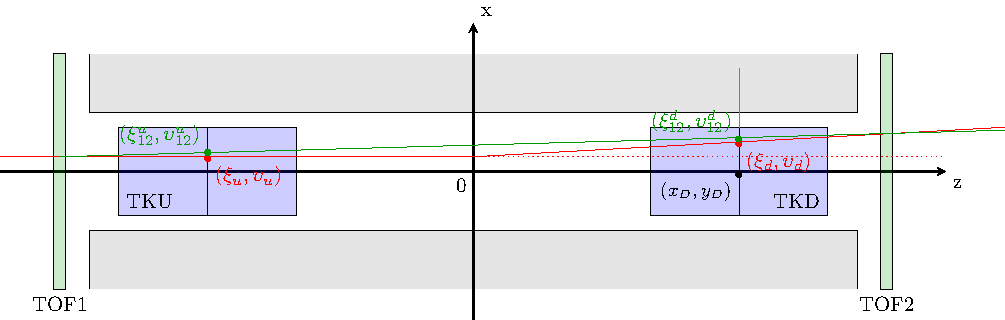
\includegraphics[width=0.95\textwidth]{alignment.pdf}
	\end{center}
	\caption{
		True path of a single particle track (red) and its path as reconstructed from the time-of-flight system (green). The position of the track at the tracker centres is represented by markers.
	}
	\label{fig:align_bl}
\end{figure}

Each TOF provided a single space point in the global coordinate system. This position was assumed to be the true position with a large uncertainty due to the limited granularity of the detector.
Trackers sampled the particle track in five different stations and this allows for the reconstruction of a straight track without any assumption made on the prior position of the tracker.
In global coordinates, on average, the track reconstructed between TOF1 and TOF2 should agree with the track reconstructed in either tracker, i.e. the mean residuals should be zero. Applying this reasoning to the unknown offset and angles yields to a system of equations for the four unknown constants~\cite{2018arXiv1805.06623T}.
The measurement of four residual distributions per tracker yields the alignment constants.
The main source of bias was the scattering in the material between TOF1 and TOF2. If the beam was not perfectly centred, particles preferentially scraped out on one side of the magnet bore, anisotropically truncating the tail of the residual distribution. The selection criteria defined above remove this effect.

Data was recorded with the superconducting magnets of the experiment turned off. High momentum beams were used to reduce the RMS scattering angle and maximise transmission.  
Each data set was processed independently. Figure~\ref{fig:runtorun} shows the alignment parameters measured for each run during a specific ISIS user cycle. The measurements were in good agreement with one another and showed no significant discrepancy: an agreement between the independent fits guaranteed an unbiased measurement of the alignment constants. The constant fit $\chi^2/\text{ndf}$ was close to unity for each fit, which indicated that there were no significant additional source of uncertainty. The optimal parameters are summarised in table\,\ref{tab:201701_constants}. 

\begin{table}[ht!]
	\centering
		\begin{tabular}{l|c|c|c|c}
			& x [mm] & y [mm] & $\alpha$ [mrad] & $\beta$ [mrad] \\
			\hline
			TKU & $-0.032\pm0.094$ & $-1.538\pm0.095$ & $ 3.382\pm0.030$ & $0.412\pm0.029$ \\
			TKD & $-2.958\pm0.095$ & $ 2.921\pm0.096$ & $-0.036\pm0.030$ & $1.333\pm0.030$
		\end{tabular}
	\caption{Summary table of the optimal alignment constants measured in the high-momentum straight-track data acquired during the 2017/01 ISIS user cycle.}
	\label{tab:201701_constants}
\end{table}

\begin{figure} [!htb]
	\centering
	\begin{minipage}[b]{.49\textwidth}
		\centering
		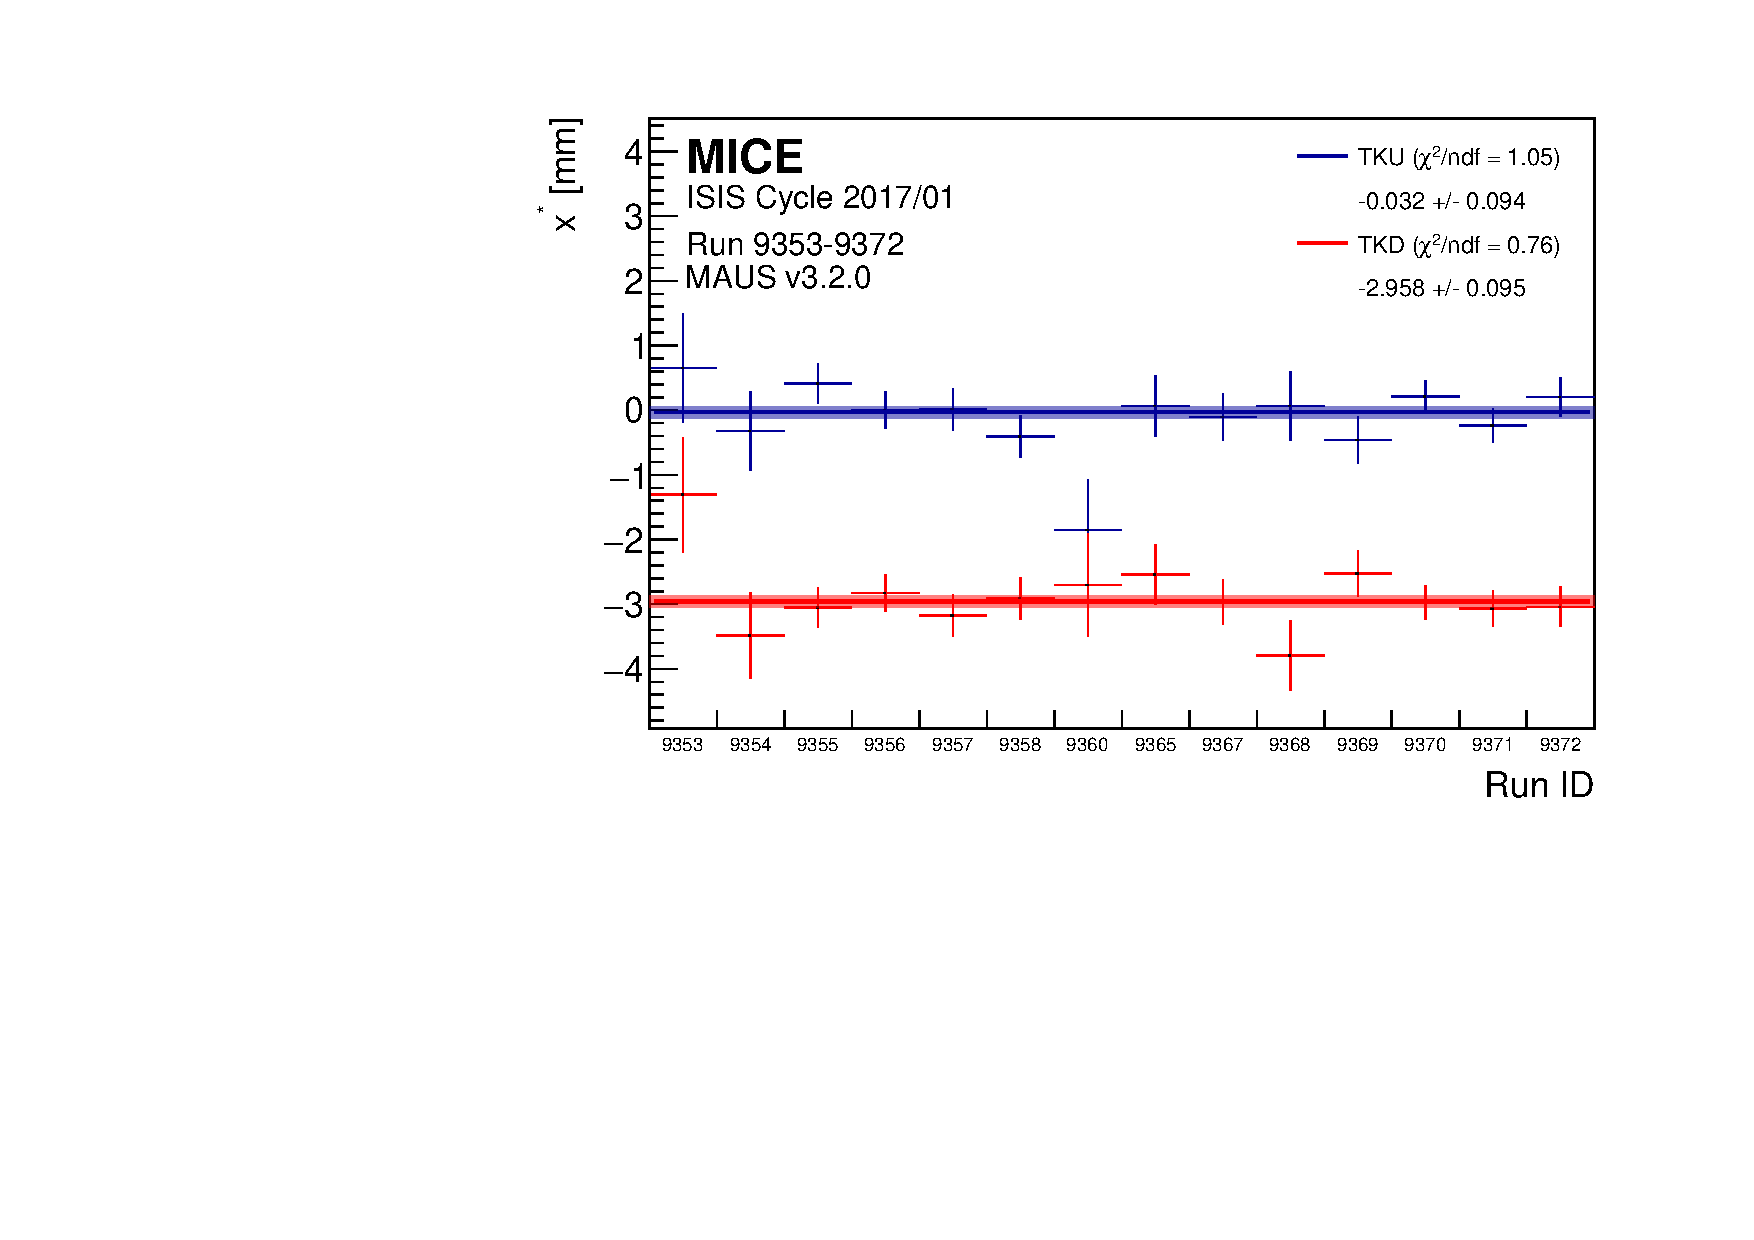
\includegraphics[width=\textwidth]{data_final/x_bestfit.pdf}
	\end{minipage}
	\hfill
	\begin{minipage}[b]{.49\textwidth}
		\centering
		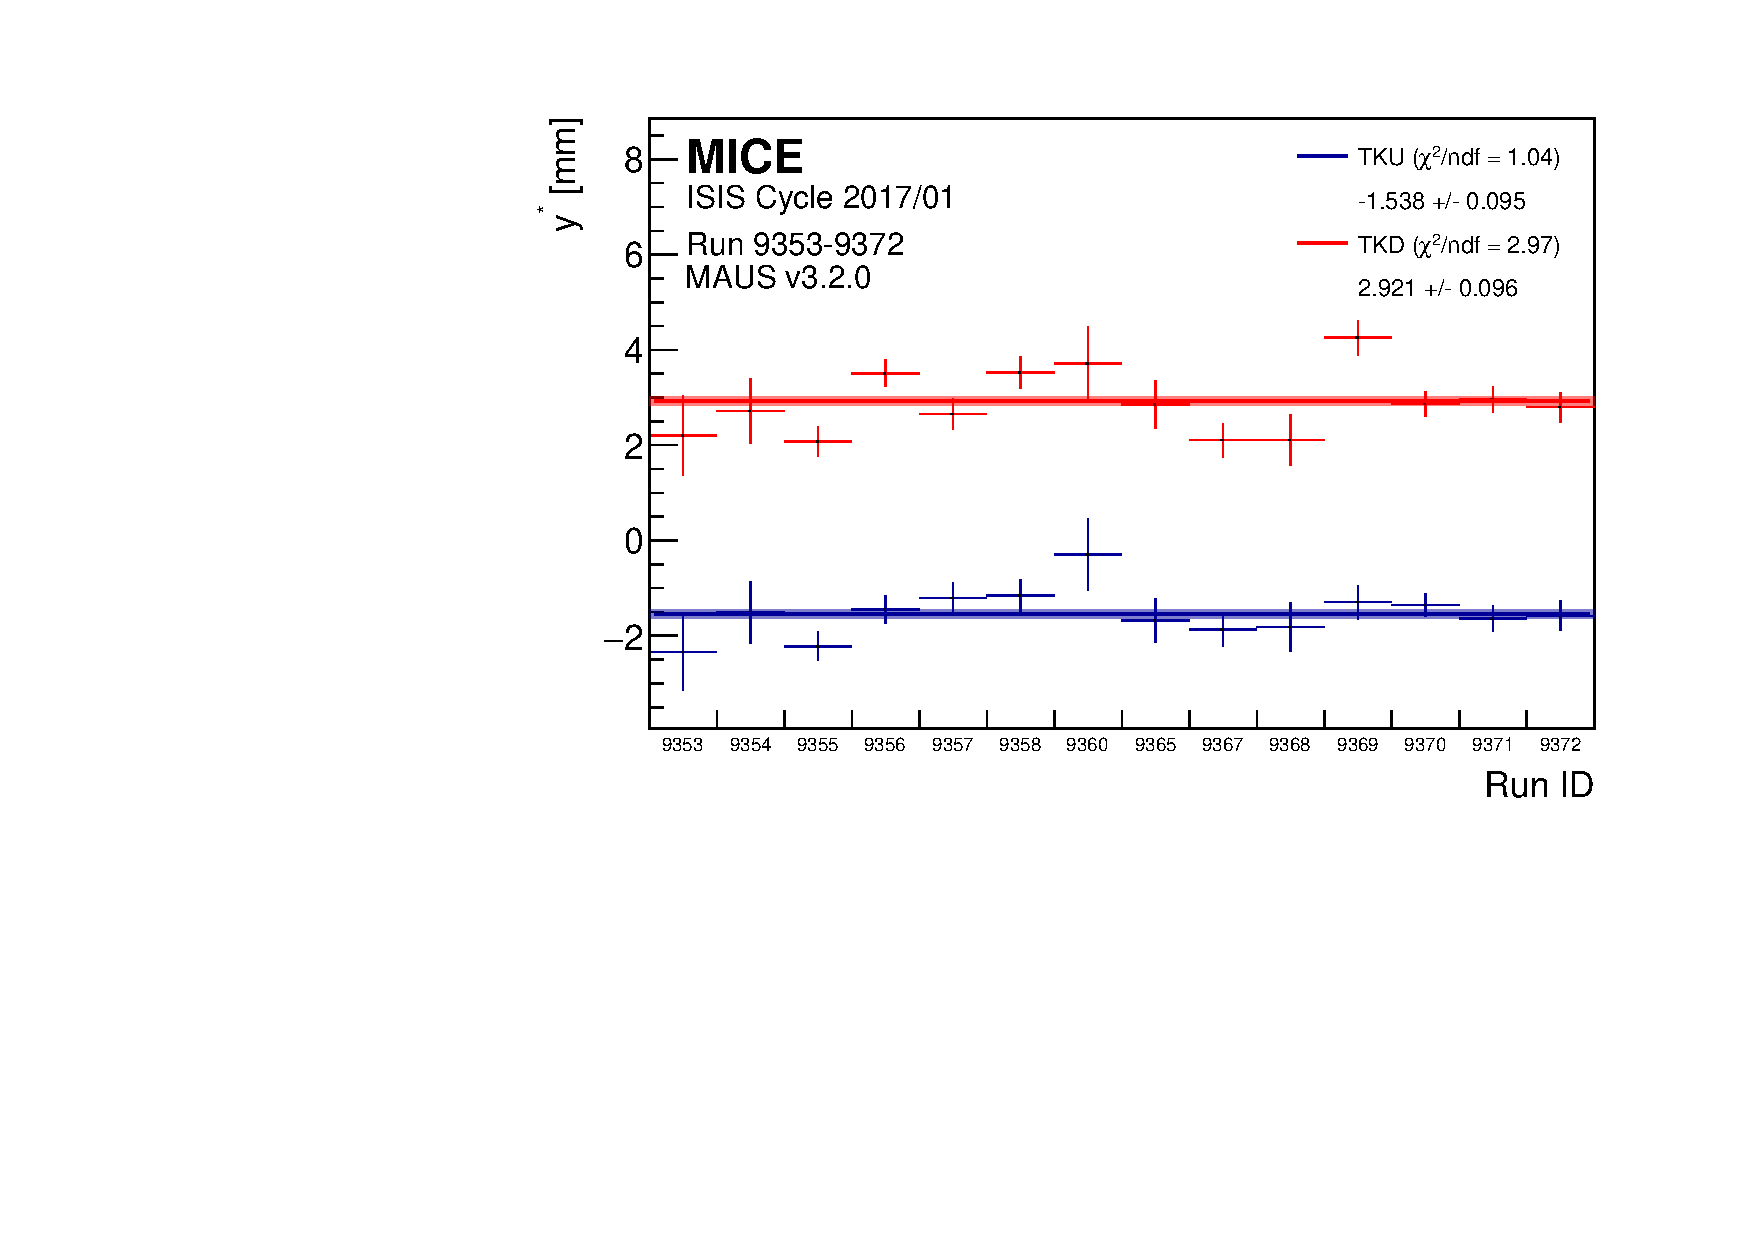
\includegraphics[width=\textwidth]{data_final/y_bestfit.pdf}
	\end{minipage}
	
	\begin{minipage}[b]{.49\textwidth}
		\centering
		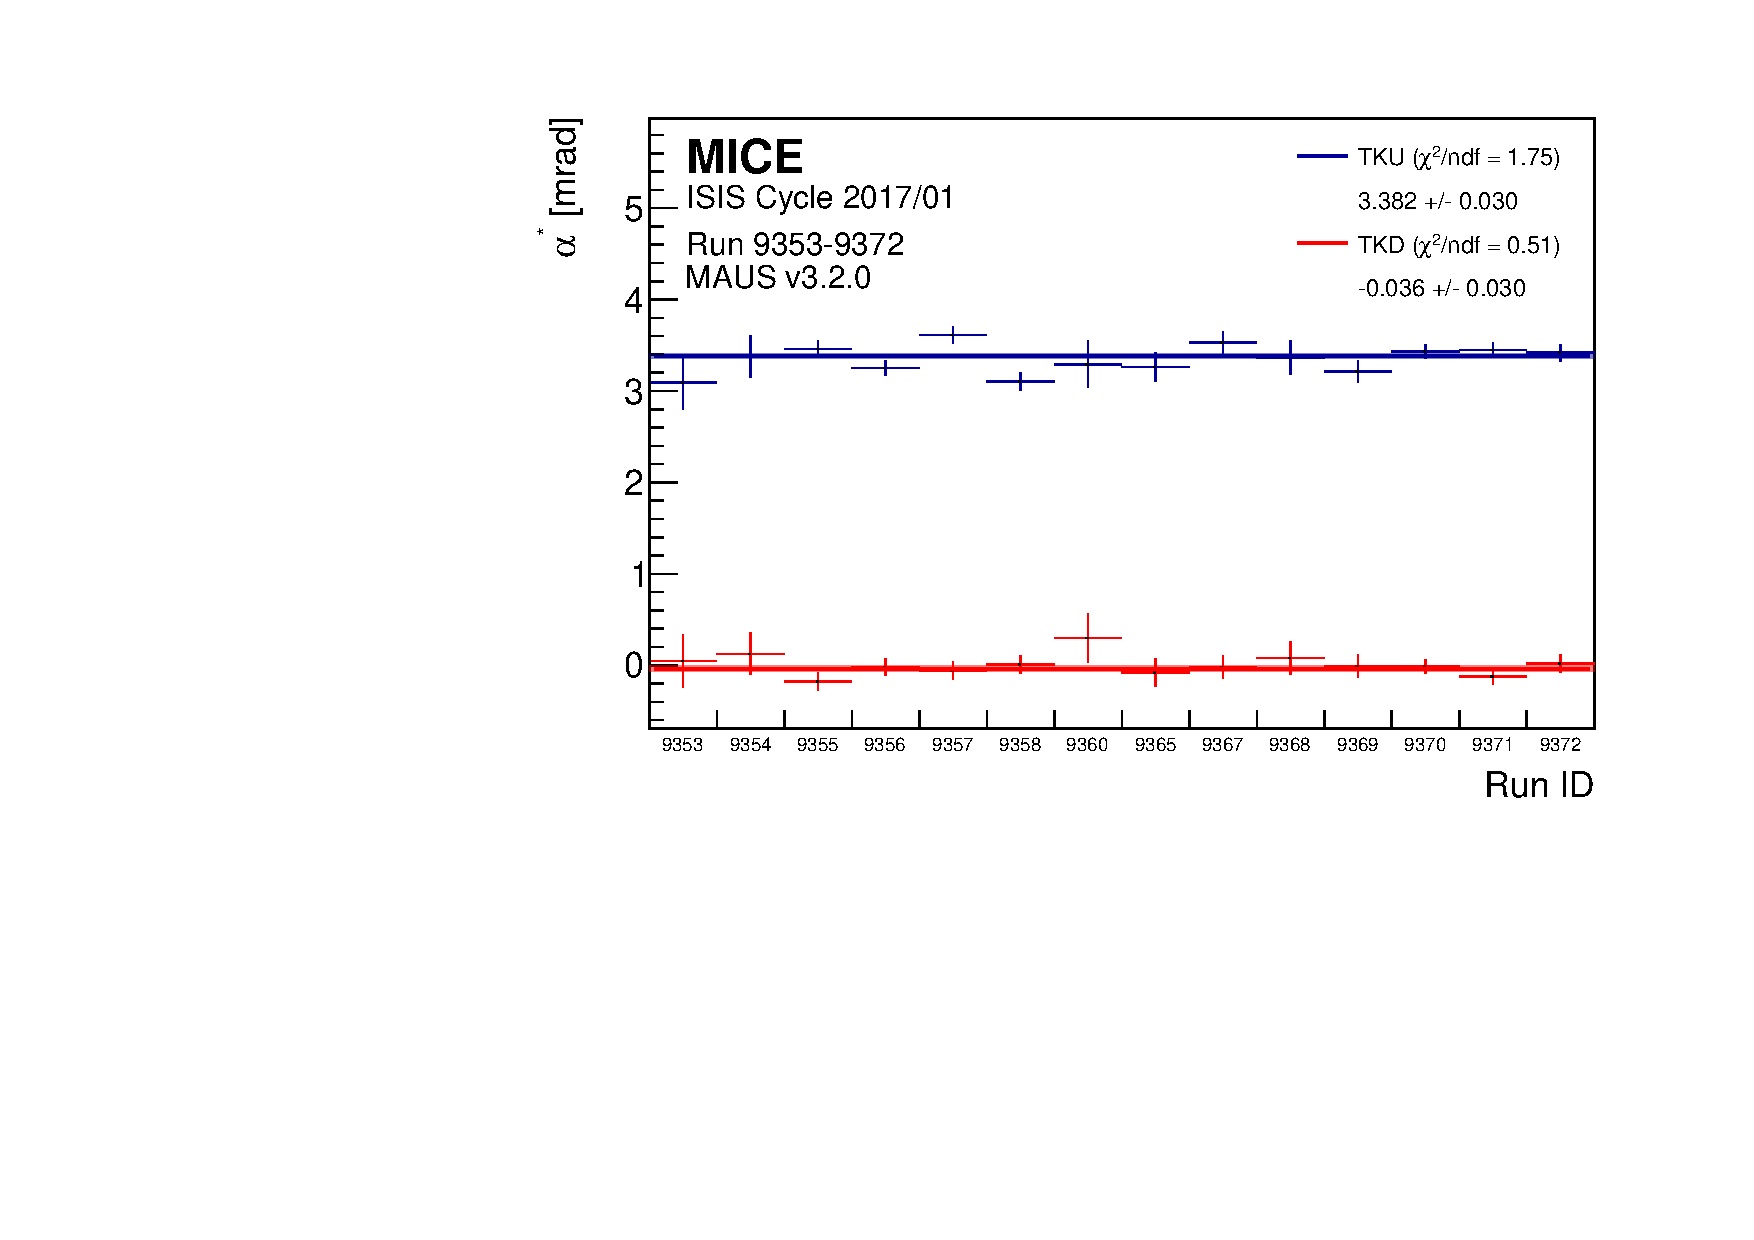
\includegraphics[width=\textwidth]{data_final/alpha_bestfit.pdf}
	\end{minipage}
	\hfill
	\begin{minipage}[b]{.49\textwidth}
		\centering
		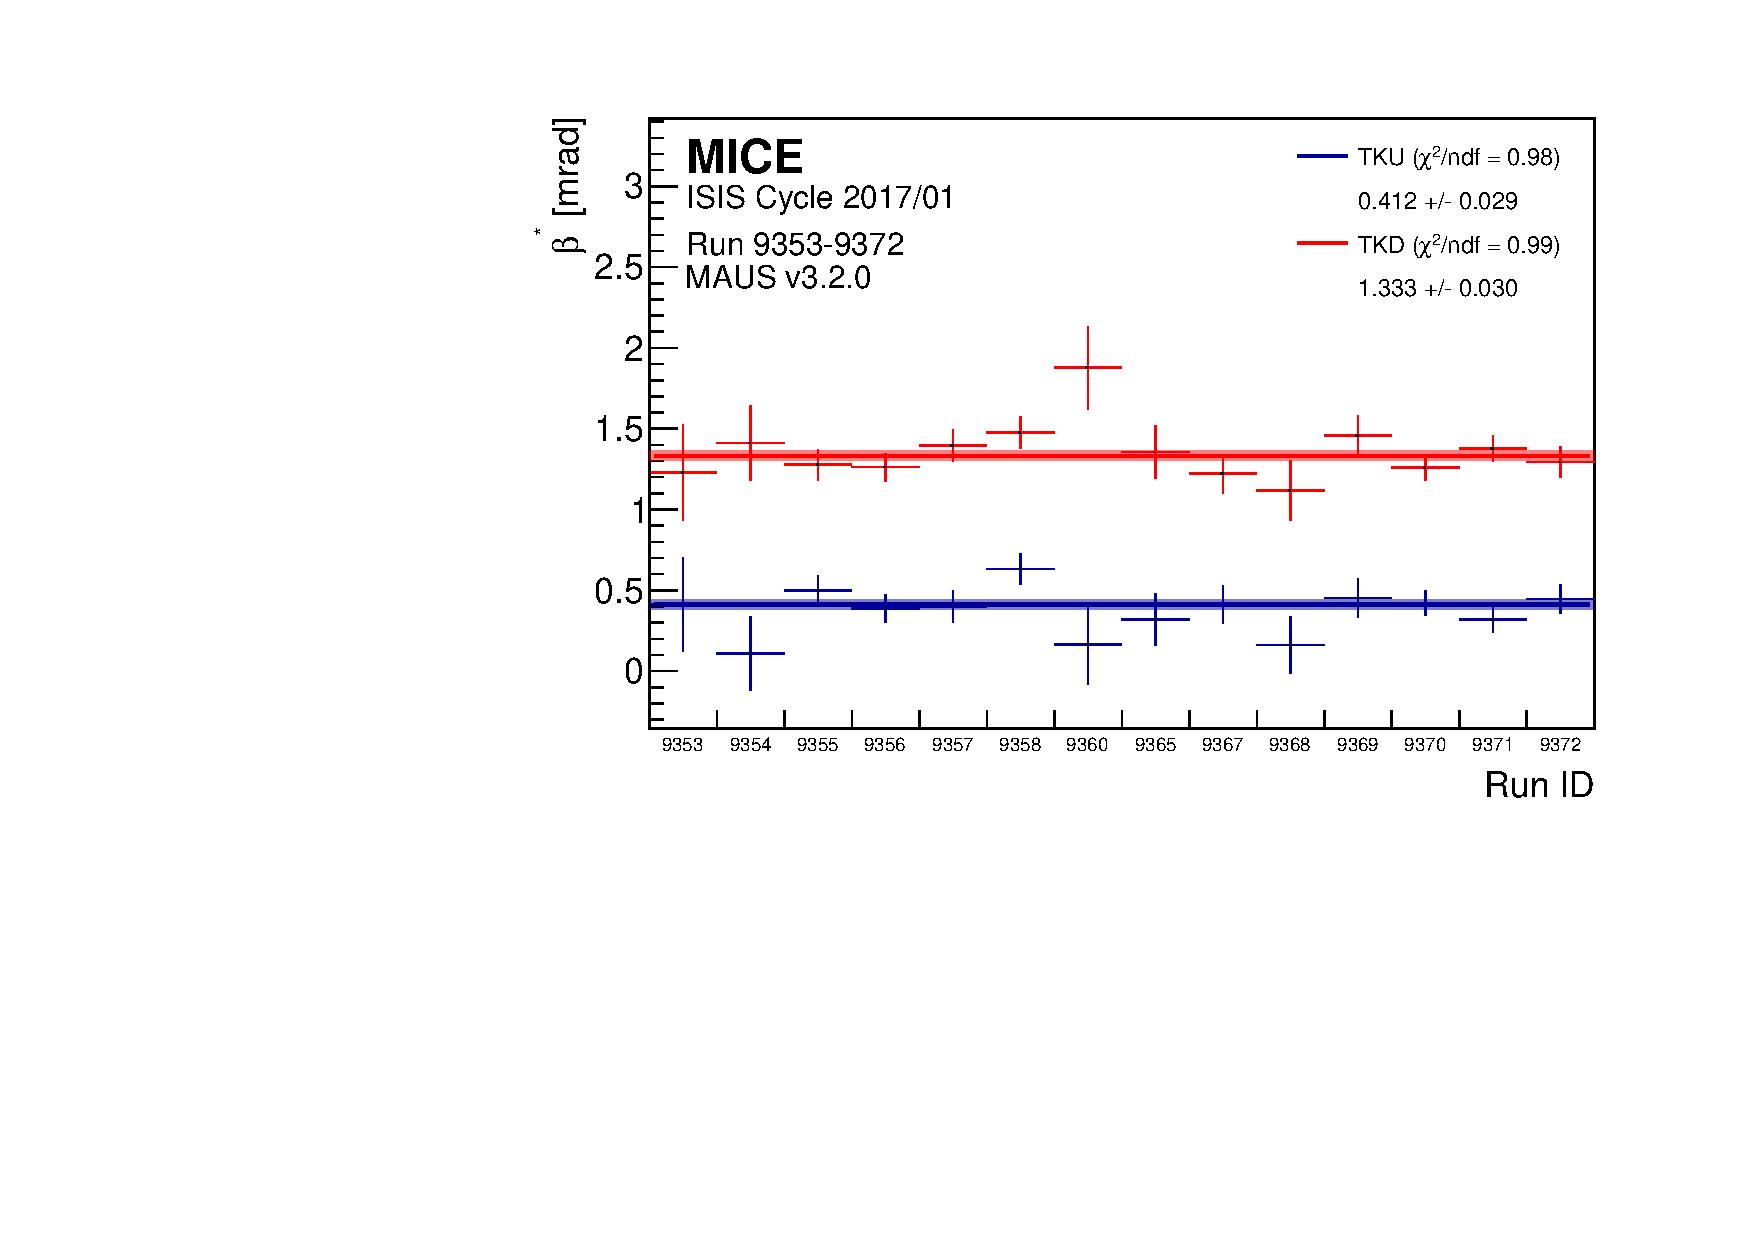
\includegraphics[width=\textwidth]{data_final/beta_bestfit.pdf}
	\end{minipage}
	\caption{Consistency of the alignment algorithm across runs acquired during the 2017/01 ISIS user cycle.}
	\label{fig:runtorun}
\end{figure}
